\section{Data Samples and Event Selection}
Trigger, DataSample, Good Run List. Mention separate 900 GeV and 2.36
TeV. 

\subsection{Vertex selection}
Show vertex distributions, discuss some group's selections on vertex.

\subsection{Removal of scraping events}
This is an example of subsection

\subsection{HCAL anomalous noise}
Commissioning studies of the CMS hadronic calorimeter performed 
during past Test Beam, Cosmic and Beam runs have identified 
sporadic noise events CMS PAPER CFT-09-019.
Intermittent anomalous signals observed so far can be grouped in two categories:
\begin{itemize}
\item{HB/HE atypical signals} Ion Feedback (typically 1-2 channels in one HPD are affected), 
HPD Noise (typically all 18 channels in one HPD are affected), RBX Noise(coherent noise affecting up to 
72 channels in one Readout Box unit);
\item{HF atypical signals} PMT window hits (Occasionally an energetic charged particle directly impinges 
upon the window of an HF PMT rather than striking a HF quartz. This results in an abnormally large 
apparent energy signal for a signal channel within the HF). 
\end{itemize}

The presence of such rare atypical signals was also confirmed in recent 2009 collision data, 
resulting in large $\etmiss$ in the event. 

Preliminary studies performed on a data sample of Mininum Bias events at $\sqrt{s}=900$~GeV 
seems to indicate that HF PMT window hits are significantly more frequent in the tail of MET
then HB/HE related noise events (for $\etmiss>14$~GeV, about 90\% of noise events attributed 
to HCAL is identified as coming from HF; see this talk for more details in 
``http://indico.cern.ch/getFile.py/access?contribId=8\&resId=6\&materialId=slides\&confId=76047'').
This can be explained considering that HF PMT window hits are beam related 
(at this stage probably beam halo muons hitting the PMT window), 
while HB/HE noise events (HPD and RBX noise) are independent from the beam activity; 
therefore the probability of overlap of an HB/HE noise event with a collision event is small.
Studies are ongoing to understand if the rate of HB/HE noise events is consistent with what 
previously observed during CRAFT09.

The list below is an attempt to summarize the 
contributions provided by different people on the identification and rejection of such atypical noise events. 

\begin{itemize}

\item{\bf HCAL studies on HBE/HE noise events} A set of algorithms have been developed by the HCAL group to 
identify and address these types of problems in the data. The methods have been tested on cosmic muon data, 
dedicated calorimeter noise data, and single beam data collected at CMS in 2008, 
as described in CMS PAPER CFT-09-019. A ``HcalNoiseSummary'' object 
is also implemented in CMSSW and it contains basic information useful to identify HB/HE noise events.
More information can be found at 
the CMS Twiki page ``HcalNoiseInfoLibrary''.
Information on HF noise events are not currently stored in the ``HcalNoiseSummary'' object.
The ``HcalNoiseSummary'' object information is not used in the current version of this note
to reject HB/HE noise events.

\item{\bf HCAL studies on HF PMT window hits} PMT windows hits within the HF are tagged by comparing 
the energies reconstructed from long and short fibers with the same ($\eta$,$\phi$) values. 
Given a pair of adjacent long and short 
fibers, with energies $E^L$, $E^S$, respectively, the fiber channels are flagged as noisy if 
(a) the maximum transverse energy $E_T^{max}$ reported by the two channels is at least 5~GeV, and (b) 
if the energy ratio R, defined as:
%
\begin{equation}
R = \frac{E^L - E^S}{E^L + E^S}
\end{equation}
%
is, in module, greater than 0.995. In this study, if at least one HF fiber channel 
is flagged by this algorithm, the event is rejected from the analysis. 
Figure~\ref{fig:hf_noise_longshortFiber} shows the scatter distributions of $E_T^L$($E_T^S$) vs $R$, 
for both data and MC, after applying the full event selection except the HF filter itself.
The HF noise events can be identified by large $E_T^L$($E_T^S$) values and $R$ values close to 1 or -1.
\\
\\
%
\begin{figure}[h!]
 \centering
 \begin{tabular}{ll}
  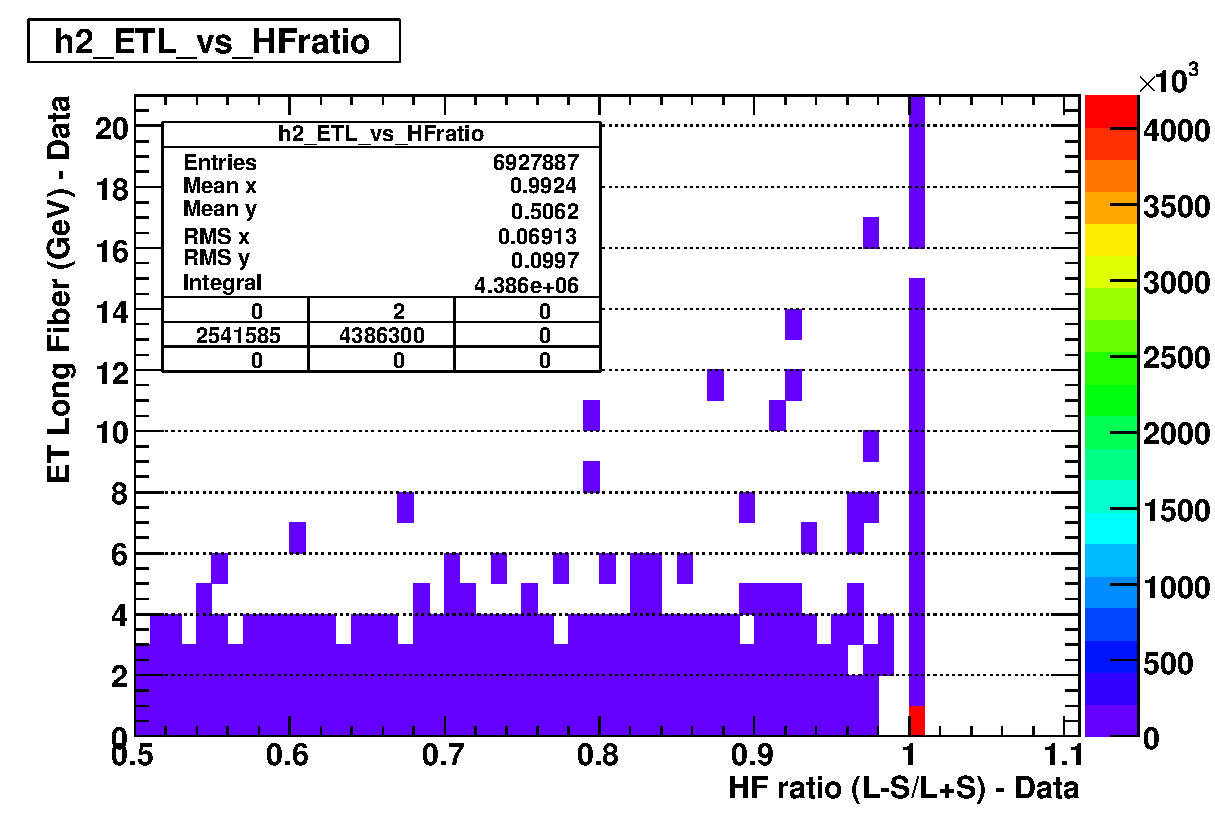
\includegraphics[width=0.5\textwidth]{plots_hcalnoise/hf_longfiberET_vs_ratio_DATA.eps} &
  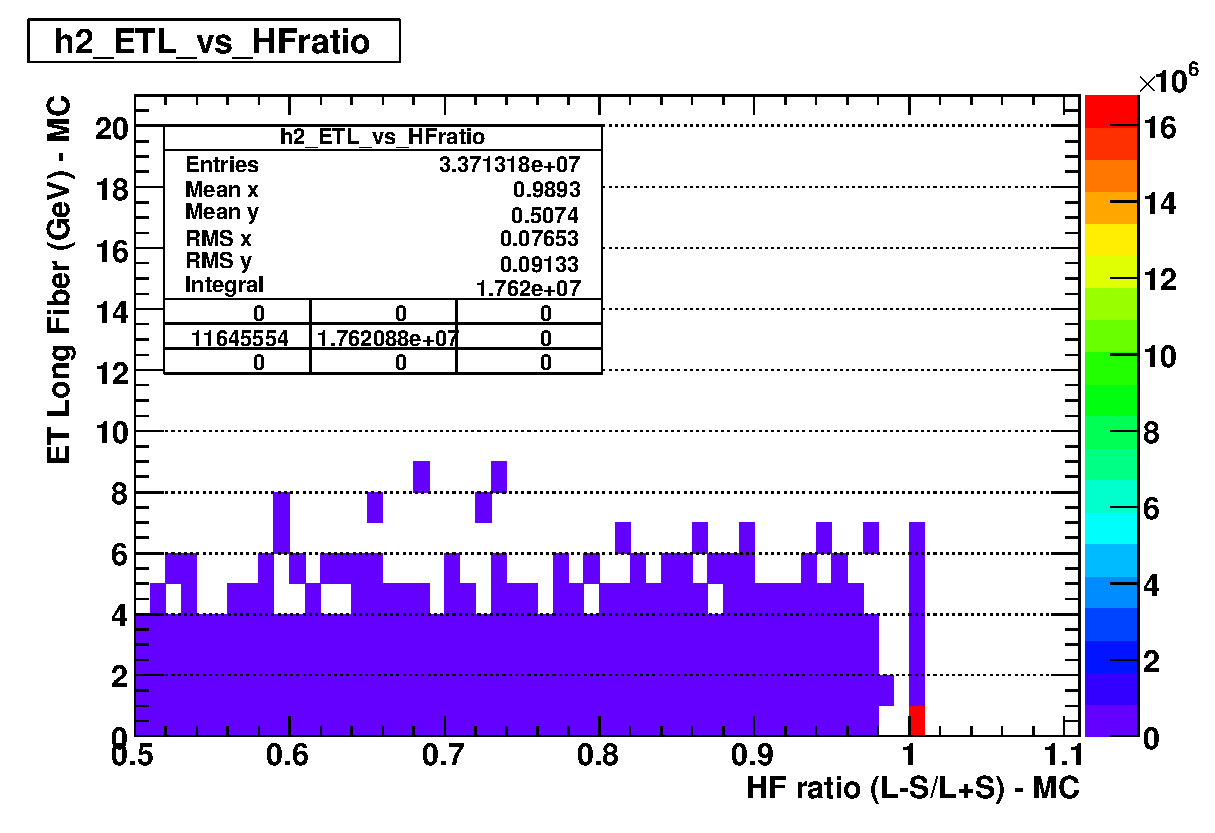
\includegraphics[width=0.5\textwidth]{plots_hcalnoise/hf_longfiberET_vs_ratio_MC.eps} \\
  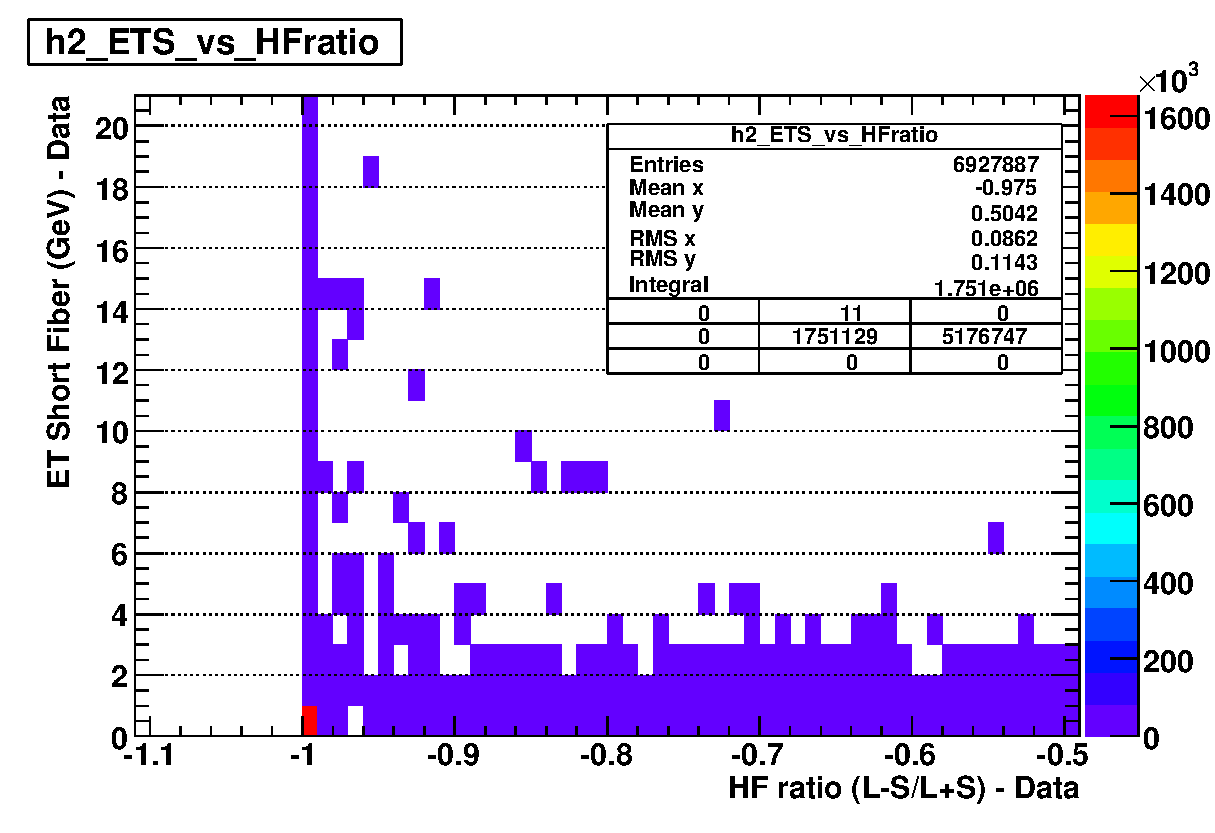
\includegraphics[width=0.5\textwidth]{plots_hcalnoise/hf_shortfiberET_vs_ratio_DATA.eps} &
  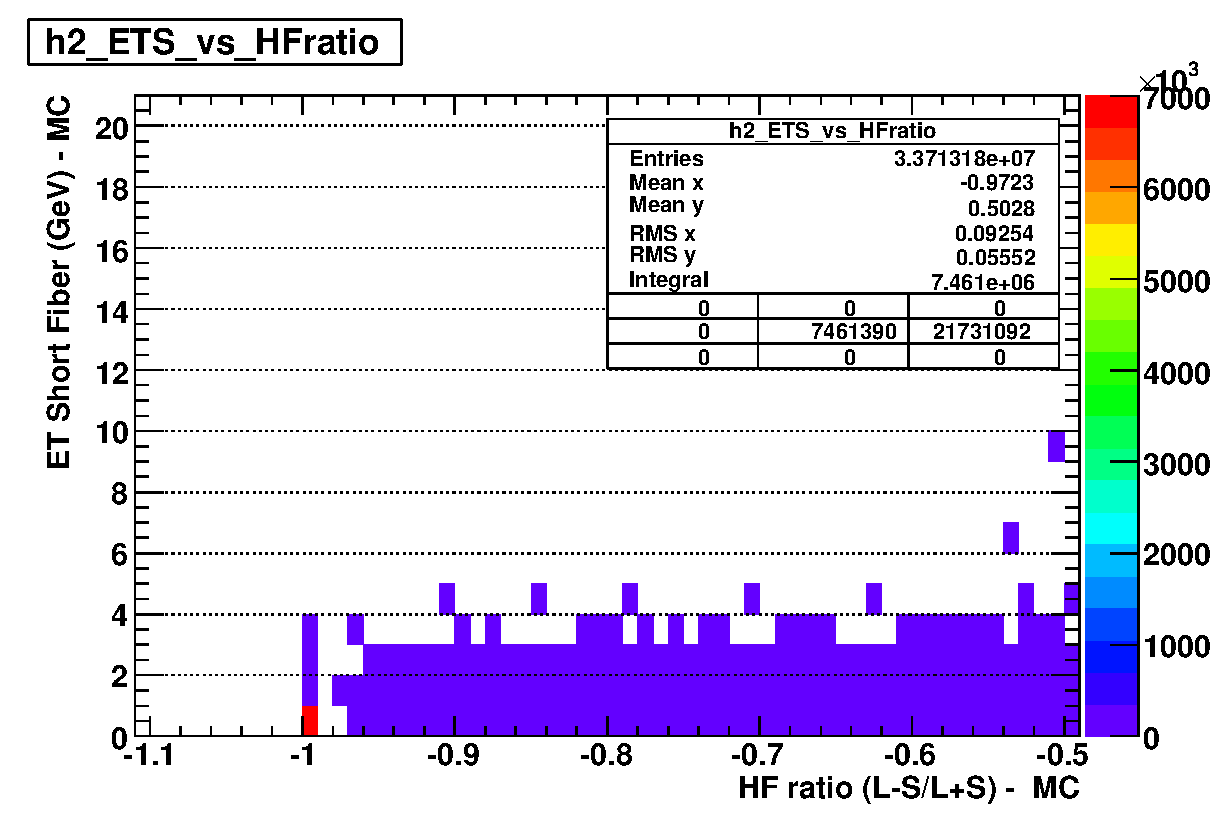
\includegraphics[width=0.5\textwidth]{plots_hcalnoise/hf_shortfiberET_vs_ratio_MC.eps} \\
 \end{tabular}
\caption{\small (Top) Scatter distribution of transverse energy in the long fibers versus $R$ for both data (Left) and MC (Right), 
and (Bottom) distribution of transverse energy in the short fibers versus $R$ for both data (Left) and MC (Right), 
after applying the full event selection except the HF filter itself. 
Plots are filled for each HF tower if either $E_L>1.2$~GeV or $E_S>1.8$~GeV. 
The x axis range is chosen in order to highlight the region where noise events appear. \label{fig:hf_noise_longshortFiber}}
\end{figure}
%

\item{\bf HCAL noise cleaning from PFMET group}
need to be added.

\end{itemize}

\subsection{ECAL anomalous noise}

This is an example of subsection

\begin{2figures}{hbtp}
  \resizebox{8cm}{!}{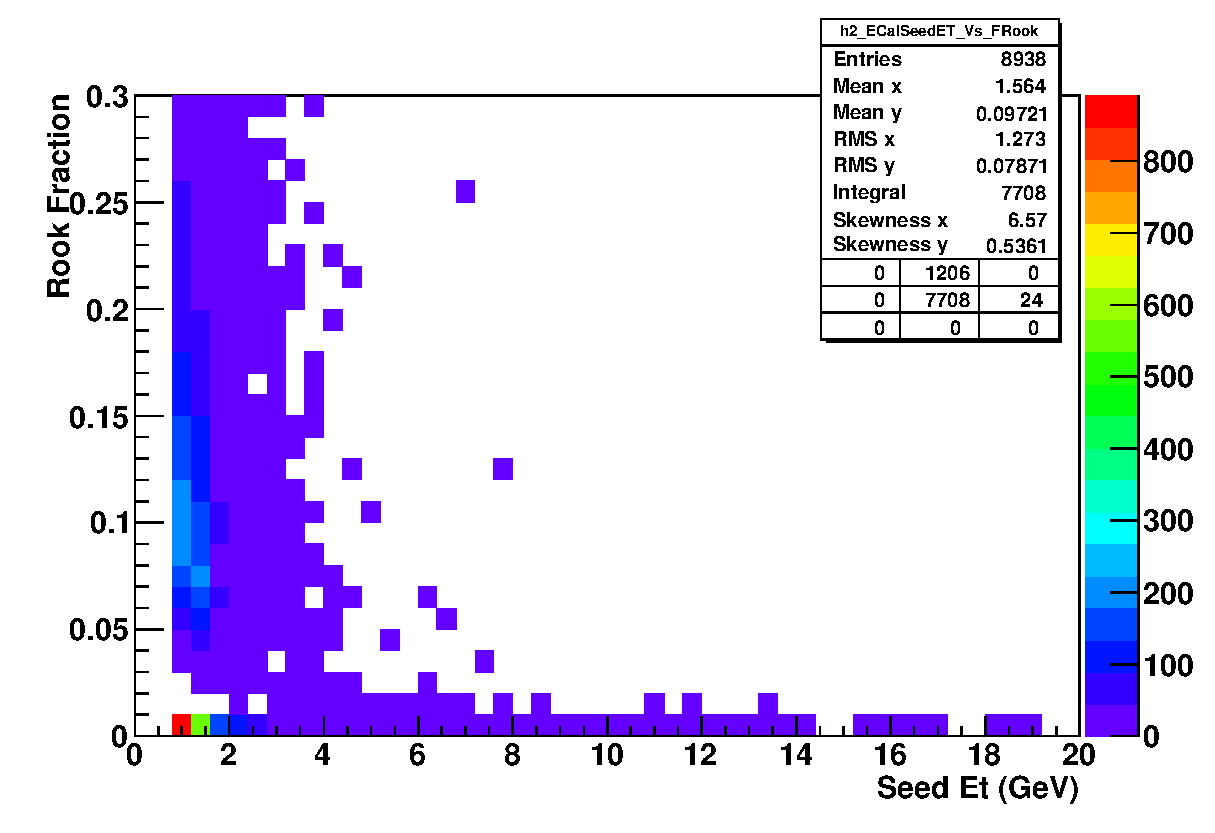
\includegraphics{plots_ecalnoise/SeedET_Frook_DATA900GeV.eps}} &
  \resizebox{8cm}{!}{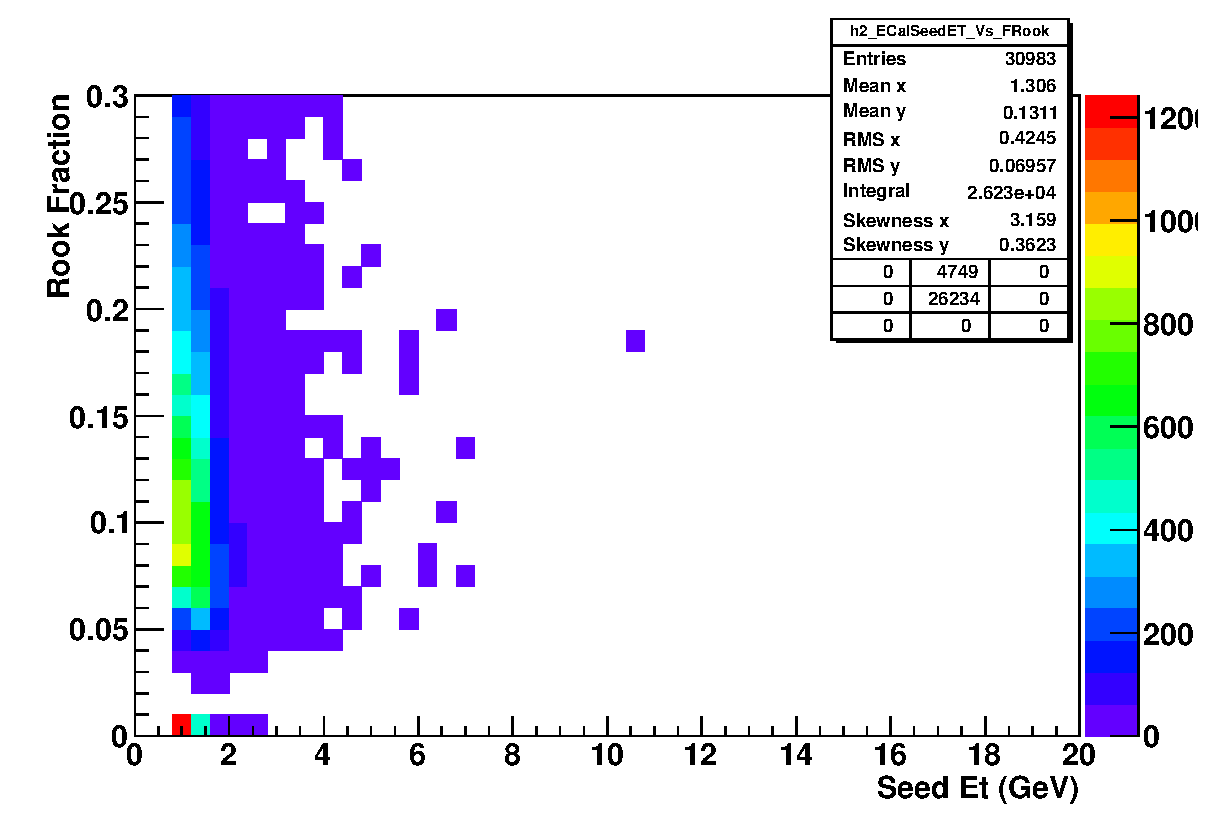
\includegraphics{plots_ecalnoise/SeedET_Frook_MC900GeV.eps}} \\
\caption{900 GeV Data Vs MC}
 \label{fig:ecal_noise_1}
\end{2figures}

Add cut efficiency table HERE.

\begin{table}[htbp]
 \label{tab:HEEPselection}
 \begin{center}
   \begin{tabular}{|lcc|lcc|} \hline
     \multicolumn{3}{|c|}{ID Variables} & \multicolumn{3}{|c|}{Isolation Variables} \\
     Variable & Barrel & Endcap & Variable & Barrel & Endcap  \\ \hline
     $H/E$  & $<0.05$ & $<0.1$ & $N_T$  & $<4$ & $<4$ \\ \hline
     $\sigma_{\eta\eta}$  & $<0.011$ & $<0.0275$ & Track iso (GeV) & $<7.5$ & $<15$ \\ \hline
     $|\Delta\eta^{trk-SC}|$ & $<0.005$ & $<0.007$ & EM iso (GeV) & $<6+0.01*E_{t}$ & $<6+0.01*E_{t}$ \\ \hline
     $|\Delta\phi^{trk-SC}|$ & $<0.09$ & $<0.09$ & HAD iso (GeV) & $<4+0.005*E_{t}$ & $<4+0.005*E_{t}$ \\ \hline
   \end{tabular}
 \caption{\small \sl HEEP electron ID and isolation criteria.
   Reconstructed electrons are associated to the
   barrel (endcaps) if $|\eta|<1.442$ ($1.560<|\eta|<2.5$).}
 \end{center}
\end{table}


\subsection{Effect of noise removal}
Here we put the $\etmiss$ distribution with base selection, after HCAL/ECAL
noise removal.

\clearpage
